\chapter{Játékmenet}

\section{Játék elkezdése}
A játék elkezdéséhez rá kell kattintanunk a barlangra. Miután rákattintottunk a barlangra az új játék megkezdéséhez választanunk kell egy karakter klasst. Ezek mind más-más játékstílussal bírnak a játékos számára. Miután kiválasztottuk a karaktert kapunk egy kezdő paklit. Ez a pakli 5 darab egyedi kártyából melyek a klass saját kártyái illetve 4 mindenki számárá elérhető kártyából áll. Ez a 4 kártya 2 Strike, 1 Draw és 1 Defend kártyából áll.

\subsection{Kasztok}
\begin{itemize}
        \item Warrior avagy a Harcos:\\\
        Agresszív támadás orientált játékstílus. Fő fókuszban a Strike kártyák álnak és ezeknek az erősítése. A klass 2 felszereléssel, és 3 varázslak kártyával rendlekezik. 
        \item Ranger avagy az Íjjász: \\\
        Hibrid kombinációja az agresszív támadás orientált és passzívabb önerősítő játékstílusnak. A Ranger kombinálja a felszereléseinek támadási előnyeit az aréna effektusok kontrolláló képességeivel. A klass 2 felszereléssel, 1 varázslattal és 2 aréna effektussal operál. 
        \item Mage  avagy a Mágus: \\\
        Varázslat orientált passzívabb játékstílus. Ereje a varázslatok erősítésében és a támadások mágiával való kombinációjában rejlik. A klass 2 varázslattal, 2 felszereléssel és 1 aréna effektussal rendelkezik.
        \item Paladin avagy a Lovag: \\\
        Passzív védelem és pajzs orientált játékstílus. A Paladin képes a pajzsát sebzésre használni.  A klass 3 varázslattal, 1 felszereléssel és 1 aréna effektussal rendelkezik.
        \item Druid avagy a Druida:\\\
        Passzív öngyógyítás és gyógyulás közbeni mágikus sebzésre épülő játékstílus. A Druid fő erőssége hogy konzisztensen tudja magát gyógyítani és támadni is egyszerre. A klass 2 varázslattal, 1 felszereléssel és 2 aréna effektussal rendelkezik.
        \clearpage
        \item Ninja  avagy a Nindzsa:\\\
        Agresszív támadás és Token generálásra épülő játékstílus. A ninja erejét a dobókései adják melyeket képes generálni illetve erősíteni kártyáiva. A klass 3 varázslattal és 2 felszereléssel rendelkezik.
        \item Necromancer avagy a Nekromanta:\\\
        Agresszív játékstílus a idézett csontváz katonákra és élet pont felhasználásra építve.
        A Nekromancer az idézett élőhalott katonájival képes nagy fizikai és mágikus sebzést kiosztani illetve életpontjait felhasználni kártyák szerzésére. A klass 2 varázslattal és 2 idézett lénnyel és 1 aréne effektussal rendelkezik.
        \item Alchemist avagy az Alkemista\\\
        Agresszív kártya generálásra épülő játékstílus. Az Alchemist fő erőssége a főzetei amikor sokrétű képességekkel rendelkeznek. A klass 3 varázslattal és 2 felszereléssel rendelkezik.
\end{itemize}

\section{Játék az arénán belül}

Amint kiválasztottuk a klasst amivel játszani szeretnénk bekerülünk az arénába. A játék körökre van osztva. A játékos kezd. Az első körben a játékos felhúz 5 lapot, 4 kezdő lapot és plusz 1 lapot amit minden kör elején felhúz. Ezeket a lapokat a játékos a köre során tudja kijátszani. A kártyák sokmindenre képesek. Vannak amelyek csak egyszerű támadás kártyák amik az ellenfelet sebzik míg mások egyszer felhasználható úgynevezett Token kártyákat hoznak létre 

Ha a játékos befejezte a kötét akkor a középen található End turn gombra kattinva lezárhatja a körét. Amint a játékos lezárta a körát az esetleges kör végi effektusok érvényesülnek majd az ellenfél köre következik. Az ellenfél a köre elején felhúzza lapjait majd kijátsza őket. Miután végzett a körével újra a játékos köre következik. Ekkor a játékos visszanyeri az akció pontjainak egy részét, a reakciópontjait illetve az esetleges kör eleji effektusok életbe lépnek. Fontos megemlíteni hogy a játékos kezében nem lehet több mint 10 kártya egyszerre.

Ez mind addig megy így ameddig a játékos le nem viszi az ellenfele életét nullára vagy pedig a játékos saját életpontjainak száma el nem éri a nullát. Ha a játékosnak sikerül az ellenfele életpontjait leredukálni nullára akkor a játékos megnyerte a csatát és tovább léphet. Ha a játékos sikertelen volt és az ellenfél leredukálta a játékos életpontjainak számát nullára akkor a játékos vesztett.

\subsection{Győzelem}
Ha a játékos győzött akkor tovább kerül a kártya választó képernyőre ahol kibővíthati a pakliját egy tetszőleges kártyával. Miután a játékos rákattintott a kivánatos kártyára a Finalize gomb megjelenik és arra kattintava a játékos visszakerül az arénába ahol folytathatja a harcolást.

\subsection{Veszítés}
Ha a játékos veszített akkor egy felugró ablak értesíti hogy vesztett és a Main Menu gombra kattintva vissza kerül a Fő menübe.

\begin{figure}[h]
        \centering
        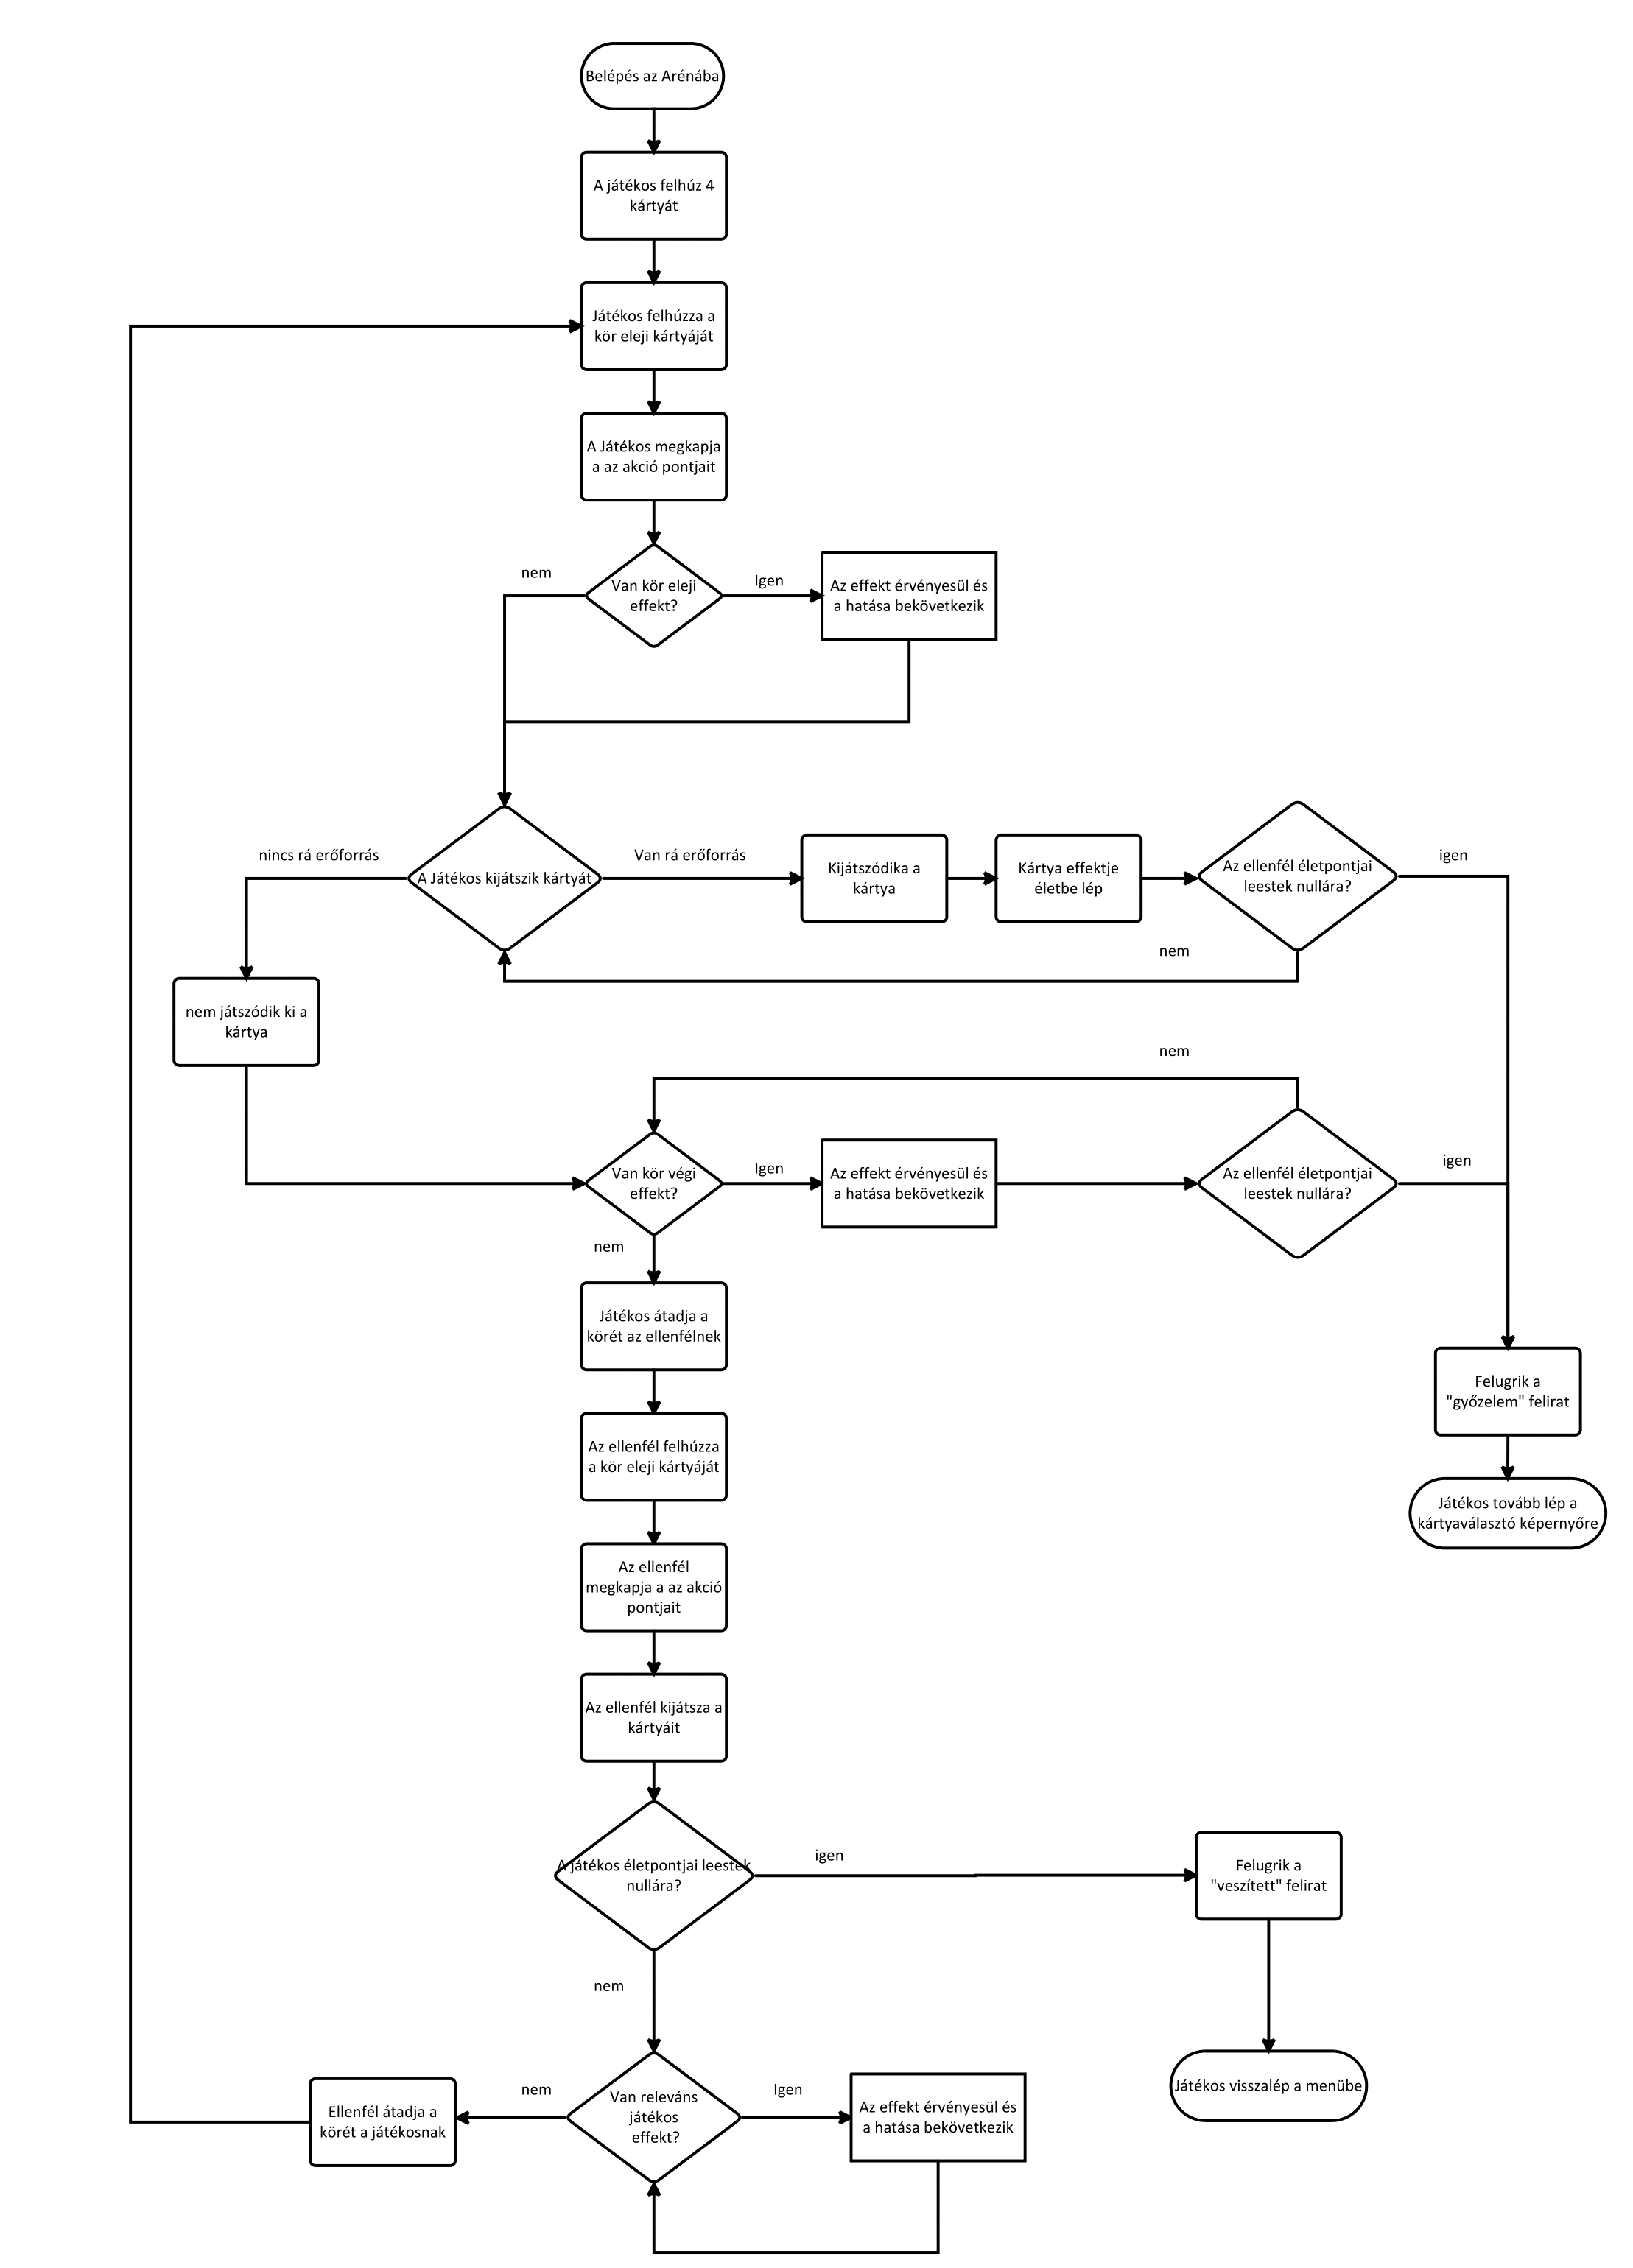
\includegraphics[width=420px,keepaspectratio]{images/Gameplay.png}
        \label{GamplayChart}
        \caption {A játékmenet folyamat ábrája}
    \hspace{1em}
\end{figure}
